\section{Results}\label{sec:results}
To investigate how the number of planets changes during a $20000$ years evolution of a solar system and how it varies with the parameter $N$(initial number of bodies). 
We varied $N$ from $500$ to $1500$ with step size $100$(thus $10$ different $N$'s). 
For each $N$, we ran only one simulation and measured the average number of planets after every $50$ years. The following results are obtained:

\begin{figure}[H]
\centering
\hspace*{-3cm}
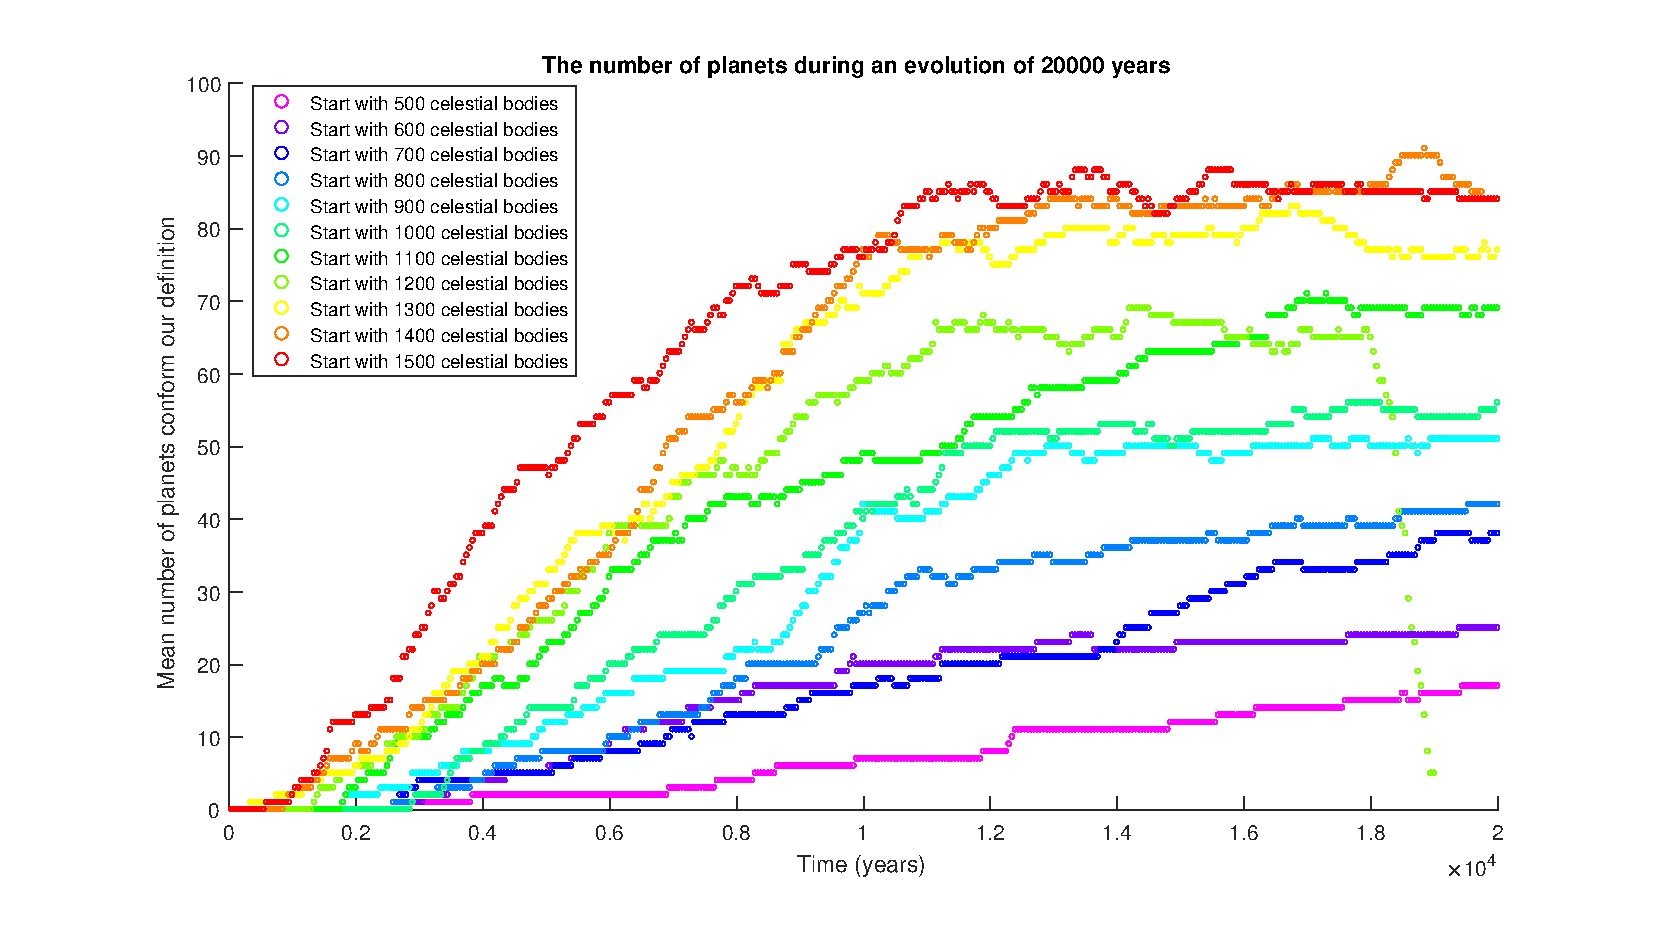
\includegraphics[scale=0.8]{AantPlanetenNieuw.eps}
\caption{Average number of planets during 20000 years of evolution, measured after each 50 years}
    \label{fig:AantPlanetenNieuw}
\end{figure}
As is shown in Figure \ref{fig:AantPlanetenNieuw}, the number of planets is a non-decreasing graph. And the more initial celestial bodies there are, the more planets are formed. This seems logical at first glance, but if we consider our own solar system, which has only 8 planets, and the number of initial celestial bodies in our early solar system was vastly greater than just $1500$, then we don't expect that the number of planets in a more realistic model will give a non-decreasing graph. Instead, because the small planetismals that are first formed will later accumulate to bigger planets, we would expect that the graph will first reach a certain peak, and then decrease after the peak. And possibly, if $N$ is large enough, the number of planets will reach to a constant that is independent of $N$. In fact, we have obtained such a graph in our earlier simulations(see Appendix), but unfortunately, the graph was a result from a miscalculation. \\

What is then the reason that the number of planets is non-decreasing? We think that is because we don't have enough initial celestial bodies, which results in less collisions and thus small planets are too far apart to make bigger planets.\\
\\
An important thing to note is the graph of $N=1200$, in which there is suddenly a decrease in the number of planets to almost zero. This is not due to the accretion we just discussed, but an error. It is observed that the momentum of the system is not conserved, which sometimes results that all bodies escaped the solar system including the sun.\\
\\
In our case where $N\leq 1500$, a larger $N$ results in a larger number of planets, we would expect that the planets formed are light and small planets. Therefore, we have made the following graphs:
%\vspace{-3cm}
\begin{figure}[H]
	\centering
	\begin{subfigure}{0.45\textwidth}
	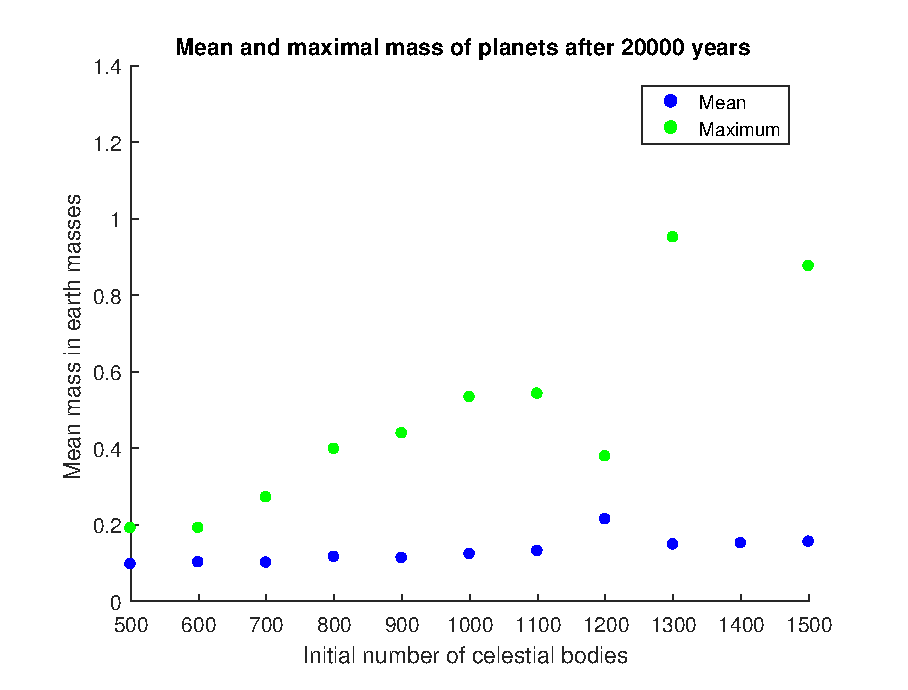
\includegraphics[width=\textwidth]{EindmassaNieuw.eps}
	\caption{Average and maximal mass of planets after 20000 years.}
	\end{subfigure}
	~
	\begin{subfigure}{0.45\textwidth}
	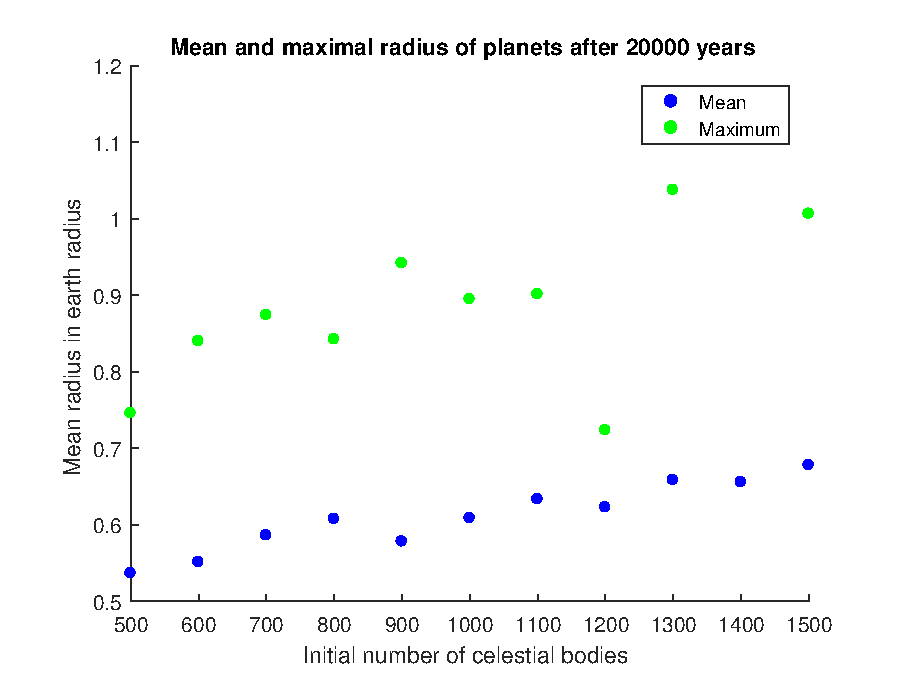
\includegraphics[width=\textwidth]{EindstraalNieuw.eps}
	\caption{Average and maximal radius of planets after 20000 years.}
	\end{subfigure}
	~
	\begin{subfigure}{0.5\textwidth}
	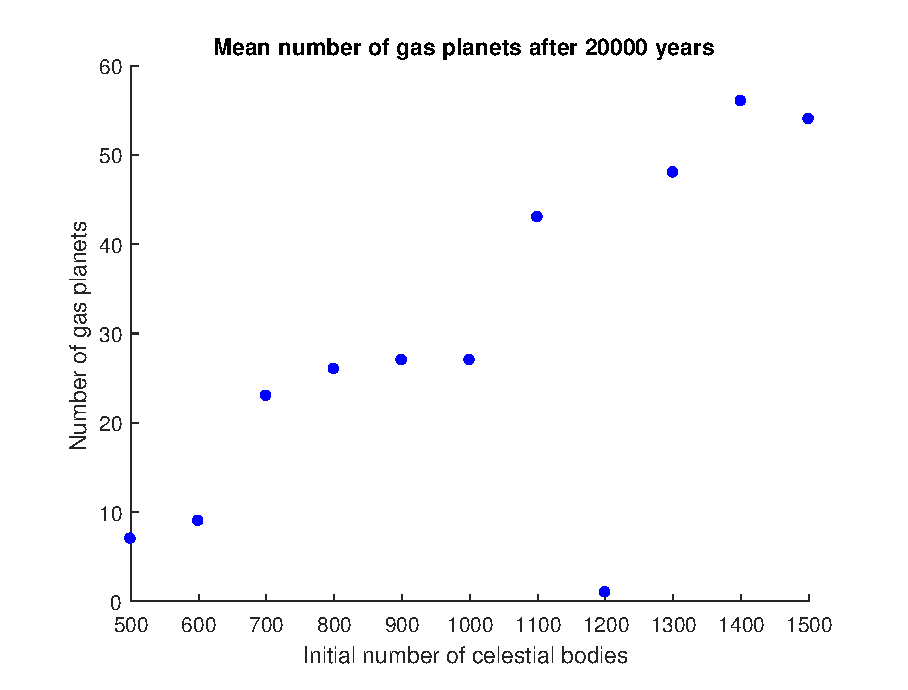
\includegraphics[width=\textwidth]{AantalGasPlaneten.eps}
	\caption{Average number of gas planets after 20000 years.}
	\end{subfigure}
	\caption{The average and maximal mass and radius of planets after 20000 years, plotted against the number of initial bodies $N$. The average mass and radius of all planets in each one of the five simulations is first calculated, and then the average of the five averages was taken for each $N$. Also, the mean number of gas planets is plotted against $N$.}
	\label{AverageMassandRadiusEnGasNieuw}
\end{figure} 
From Figure \ref{AverageMassandRadiusEnGasNieuw}, we see that the mean mass of all planets are roughly the same independent of $N$, and the heaviest planet is about 1 earth mass. For the mean radius, we see that it depends roughly linear to $N$. This is in accordance with the increasing number of gas planets we observed.